La détection se fait en trouvant les points où la puissance du signal dépasse un seuil défini (1\% de la puissance maximale). Les indices correspondants sont ensuite convertis en temps, fournissant ainsi les instants de début et de fin de chaque note. Les notes d'une durée inférieure à une seconde sont éliminées pour garantir la qualité des données. 
Fig.\ref{fig:Note_Detection} est le signal avec les notes détectées(partie rouge).
\begin{figure}[htb]
    \centering
    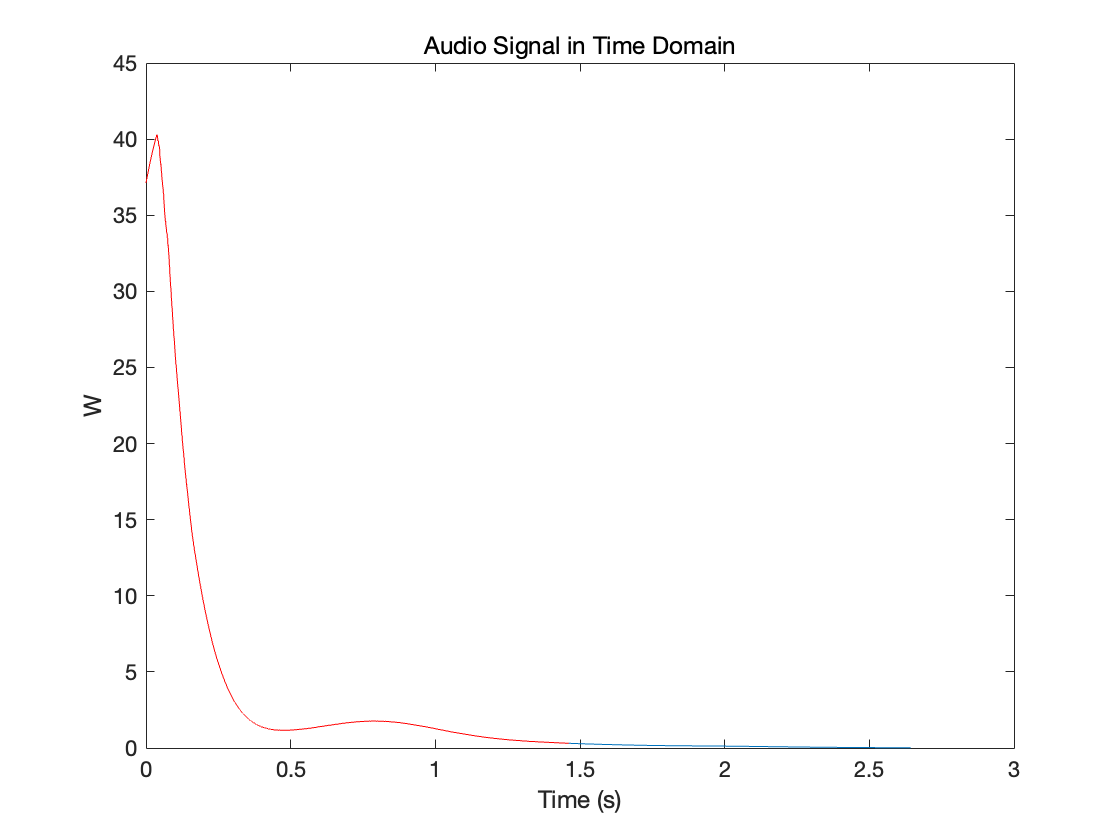
\includegraphics[width=0.8\textwidth]{signal_with_note_detected.png}
    \caption{Exemple signal avec les notes détectées}
    \label{fig:Note_Detection}
\end{figure}